\documentclass[11pt]{scrreprt}
\usepackage[T1]{fontenc}
\usepackage[utf8]{inputenc}
\usepackage[french]{babel}
\usepackage[scale=0.775]{geometry}
\usepackage{lmodern}
\usepackage[ilines]{scrpage2}
\usepackage[pdftex, bookmarks=true, hidelinks]{hyperref}
\usepackage{graphicx}
\usepackage{tocbibind}
\usepackage{chngcntr}
\usepackage{tabularx}
\usepackage{float}
\usepackage{scrhack}
\usepackage{ulem}
\usepackage{mdframed}

\tolerance=1
\emergencystretch=\maxdimen
\hyphenpenalty=10000
\hbadness=10000

\counterwithout{figure}{chapter}
\counterwithout{table}{chapter}
\pagestyle{scrheadings}

\usepackage[table]{xcolor}
\definecolor{lightgray}{gray}{0.9}
\let\oldtabularx\tabularx
\let\endoldtabularx\endtabularx
\renewenvironment{tabularx}{\rowcolors{2}{white}{lightgray}\oldtabularx}{\endoldtabularx}

\let\oldtabular\tabular
\let\endoldtabular\endtabular
\renewenvironment{tabular}{\rowcolors{2}{white}{lightgray}\oldtabular}{\endoldtabular}

% clear head and foot
\clearscrheadings
\clearscrplain
\clearscrheadfoot

\cefoot[\textsc{Mighty Beards Studio}{\textsc{Mighty Beards Studio}}
\cofoot[\textsc{Mighty Beards Studio}{\textsc{Mighty Beards Studio}}
\lefoot[]{}
\lofoot[]{}
\refoot[\thepage]{\thepage}
\rofoot[\thepage]{\thepage}

\begin{document}

    \renewcommand{\labelitemi}{$\bullet$}
    \renewcommand{\labelitemii}{$\circ$}
    %%%%%% TITLE PAGE %%%%%%%%%%%%%%%%%%%
    \begin{titlepage}
        \begin{center}
            ~\\[1.5cm]
            
\includegraphics[width=7.5cm]{images/blitzlogo.png}
            ~\\[1.5cm]

            %\textsc{\LARGE Mighty Beards Studio}\\[1.5cm]

            \textsc{\Large Projet d'AAE}\\[0.5cm]

            % Title
            \rule{\textwidth}{1pt} \\[0.4cm]
            \Huge{\textsc{Blitz}}\\ \large{Clone du jeu Wazabi}\\[0.4cm]

            \rule{\textwidth}{1pt} \\[1.5cm]

            % Authors
            \textsc{Javier Lethé - Matteo Taroli - Przemyslaw Gasinski}

            \vfill

            {\large \today}
            \vfill
        \end{center}
    \end{titlepage}
    \pagenumbering{gobble}
    \tableofcontents
    \pagebreak
    \pagenumbering{arabic}

    \setlength{\parskip}{3mm}
    %	#	#	#	#	#	#	#	#	#	#	#	#	#	#	#	#	# Document

    \chapter{Introduction}
    Wazabi est un jeu de dés et de cartes dont le but est de se débarrasser de tous ses dés. Nous avons dû, dans le cadre du cours de mise en situation professionnelle, implémenter un clone de ce jeu sur une période d'une semaine. Le thème de notre clone est la 2\ieme Guerre Mondiale et s'appelle \textsc{Blitz}, diminutif de \og Blitzkrieg\fg{}.

    Un des buts de ce projet étant de se rapprocher le plus possible de l'expérience professionnelle, certaines contraintes nous ont été imposées. Entre autres, le projet devait être développé en utilisant les technologies EJB et JSP, avec la possibilité d'utiliser d'autres technologies telles que Bootstrap, JavaScript et Ajax. Il nous a aussi été demandé de procéder de manière itérative, ce que nous avons fait en procédant par Usecase. Enfin, nous étions divisés en groupes de 4, qui ont été formés par les chefs d'équipe sur base de CV anonymes.

    Nous avons divisé le travail de la manière suivante: deux personnes se sont concentrées sur le back-end (la partie EJB) et deux sur le front-end (JSP). Malheureusement, un membre du groupe a décidé d'arrêter le projet en cours de route. De ce fait, nous avons dû re-distribuer afin de pouvoir continuer à avancer.

    Le délai assez court pour réaliser ce projet à trois ne nous a malheureusement pas permis de rendre un travail aussi propre que nous l'aurions souhaité. Par exemple, nous avons pensé à implémenter des patrons de conception supplémentaires par exemple pour la gestion des effets de cartes, améliorer l'interface ou encore un timer permettant de lancer le jeu après 30 secondes.
    Dans la suite de ce rapport, nous allons présenter les détails du programme développé.

    \chapter{Analyse}
    \section{Diagramme de navigation}
    Le parcours de l'utilisateur dans \textsc{Blitz} se fait selon le diagramme suivant :

    \begin{table}[H]
        \centering
        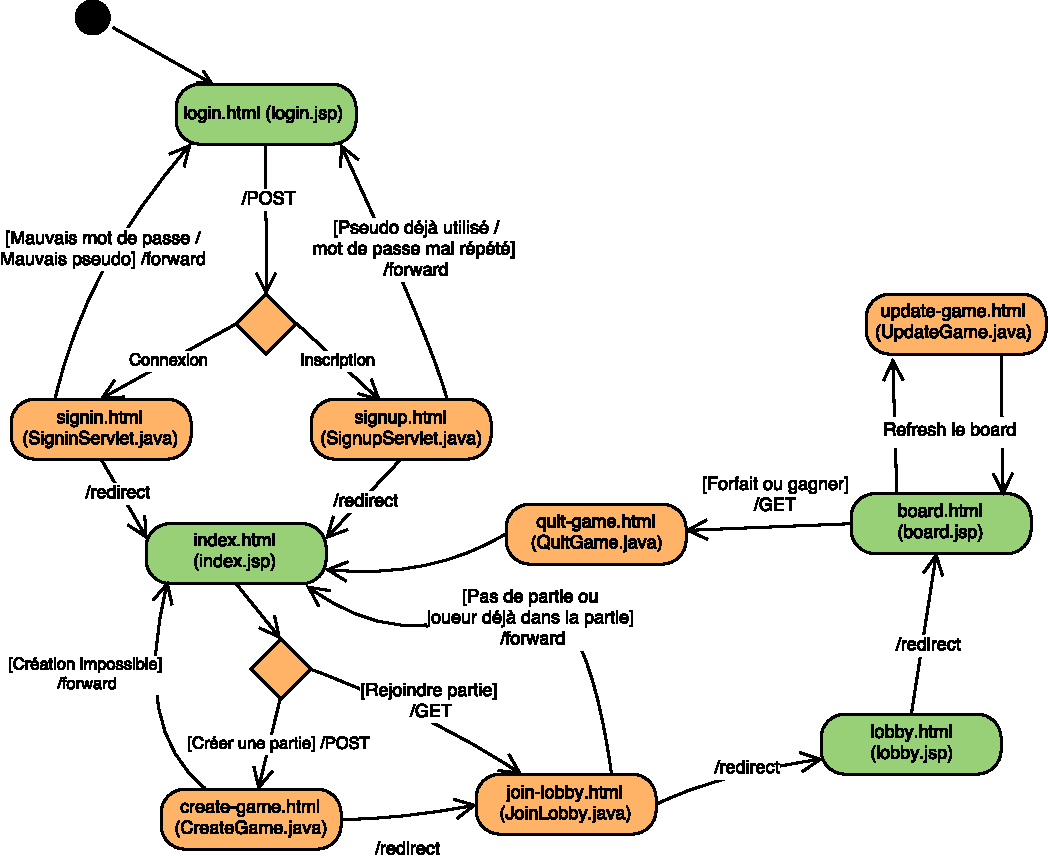
\includegraphics[width=\textwidth]{images/diag-nav.pdf}
        \caption{Diagramme de navigation}
    \end{table}

    \section{Scénario nominal \og Rejoindre une partie\fg}

    L'utilisateur étant déjà connecté, il rejoint une partie selon le scénario suivant :

    \begin{table}[H]
        \begin{tabularx}{\textwidth}{X|X}
            1. Le joueur clique sur le bouton \og Rejoindre une partie \fg{} & \\
            & 2. Le système vérifie si une partie est déjà lancée \\
            & a.1 Le système envoie le joueur vers le lobby.\\
            & a.2 Le nombre de joueurs minimal étant atteint, le jeu est lancé\\
        \end{tabularx}
    \end{table}

    \chapter{Tests}

    \section{Tests unitaires}
    Les tests unitaires de Blitz se trouvent dans le projet \og BlitzTests\fg{} et testent la classe GameUcc. Celà nous a permis de régler un nombre conséquent de bugs dans la partie EJB, ce qui n'empêche malheureusement pas certaines actions de mal fonctionner une fois appelées par l'utilisateur.

    \section{Test fonctionnels}
    \subsection{Connexion}
    \begin{table}[H]
        \begin{tabularx}{\textwidth}{X|X}
            1. Cliquer sur le bouton \og Connexion / Inscription\fg{} situé en haut à droite. & \\
            & 2. Un popup apparait proposant de s'inscrire ou de se connecter. \\
            3. Dans la partie de droite, entrer \og ol\fg{} comme nom d'utilisateur et \og ol \fg{} comme mot de passe. & \\
            & 4. Le système vérifie que l'utilisateur existe et que le mot de passe est correct et renvoie le joueur sur la page d'accueil. \\
            5. Cliquer sur le bouton \og Déconnexion\fg{}. & \\
            6. Cliquer à nouveau sur le bouton \og Connexion / Inscription\fg{}. & \\
            & 7. Le popup réapparait \\
            8. Dans la partie de droite, entrer \og ol\fg{} comme nom d'utilisateur et \og mauvaisMdp \fg{} comme mot de passe. & \\
            & 9. Le système vérifie que l'utilisateur existe et que le mot de passe est correct et affiche l'erreur \og Nom d'utilisateur ou mot de passe incorrect\fg{} et reste sur le popup.\\
        \end{tabularx}
    \end{table}

    \subsection{Création de partie}
    \begin{table}[H]
        \begin{tabularx}{\textwidth}{X|X}
            1. En partant de la page d'accueil, cliquer sur le bouton \og Créer une partie\fg{}. & \\
            & 2. Un popup apparait permettant d'entrer le nom de la partie.\\
            3. Entrer \og test\fg{} en tant que nom de partie. & \\
            4. Cliquer sur le bouton \og OK\fg{}. & \\
            & 5. Le système renvoie vers le lobby de la partie. \\
            6. Attendre d'autres joueurs et joueur. & \\
        \end{tabularx}
    \end{table}

    \subsection{Jeu}
    \begin{table}[H]
        \begin{tabularx}{\textwidth}{X|X}
            1. Attendre que ce soit
        \end{tabularx}
    \end{table}

    \chapter{Architecture}
    La partie EJB est découpé en différentes parties comme suit :
    \begin{description}
        \item[dao]\hfill \\ Contient le DAO permettant l'accès aux tables de la base de données.
        \item[daoImpl]\hfill \\ Contient les DAO implémentés permettant l'accès à une table précise selon l'entité.
        \item[domaine]\hfill \\ Contient les différents objets formant l'application.
        \item[usecases]\hfill \\ Contient les interfaces correspondantes aux usecases. Ces interfaces sont le seul lien entre la partie EJB et la partie JSP.
        \item[usecasesImpl]\hfill \\ Contient les implémentations des interfaces Usecases.
        \item[utils]\hfill \\ Contient les classes offrant des méthodes de vérification, appelées par les autres classes.
    \end{description}

    La partie JSP est quant à elle découpée de cette façon :

    \begin{itemize}
        \item Partie Java
        \begin{description}
            \item[filters]\hfill \\ Contient les filtres gérant les requêtes utilisateurs. Permet de rediriger l'utilisateur en cas d'erreur et de vérifier l'utilisation des cookies.
            \item[game]\hfill \\ Contient les servlets Java gérant une partie.
            \item[servlets]\hfill \\ Contient les servlets gérant le reste de l'application.
        \end{description}
        \item Partie Web
        \begin{description}
            \item[css]\hfill \\ Contient le css régissant le style de l'interface du programme.
            \item[images]\hfill \\ Contient les images utilisées dans l'interface.
            \item[js]\hfill \\
        \end{description}
    \end{itemize}
    \chapter{Notes}
    Parler du pattern
    de la table dés
    des inchoerences du xml,

    \chapter{Manuels}
    \section{Manuel d'installation}
    Les constantes sont dans un fichier xml, situé a Blitz/BlitzEJB/ejbModule/blitz.xml.

    \subsection{Instalation avec Eclipse}
    \begin{enumerate}
        \item Créer un schéma nommé \og blitz\fg{} dans la base de données.
        \item Importer le projet dans éclipse.\footnote{Il est supposé que Wildfly est déjà configuré, ainsi que la JDK.}
        \item Click droit sur le serveur
        \item Cliquer sur \og Add and Remove\fg{}
        \item Ajouter \og BlitzEAR\fg{}
        \item Cliquer sur \og Full Publish\fg{}
        \item Lancer le serveur
    \end{enumerate}
    \subsection{Installation sans Eclipse}
    \begin{enumerate}
        \item Créer un schéma nommé \og blitz\fg{} dans la base de données.
        \item Mettre Blitz.EAR dans le dossier suivant JBOSS\_HOME/server/your config>/deploy folder.
    \end{enumerate}

    \section{Manuel d'utilisation de Toastr}
    Pour afficher les notifications aux joueurs, nous utilisons Toastr.js (\url{https://codeseven.github.io/toastr}), qui est un plugin de jQuery. L'utilisation que nous en faisons est assez basique, la seule méthode à connaitre est la suivante : toastr.into();

    Cette méthode fonctionne de la façon suivante :

    \begin{itemize}
        \item toastr.info(\og Message\fg)\\ Affiche un Toast contenant un message à l'utilisateur.
        \item toastr.info(\og Titre\fg, \og Message\fg)\\ Affiche un Toast contenant un message et un titre à l'utilisateur
    \end{itemize}
    \section{Manuel d'utilisation}
    \subsection{Comment accéder au jeu?}
    Pour jouer sur une machine locale, tapez dans le browser \og \url{localhost:8080/Blitz}\fg{} (sans les guillemets).

    Une fois connecté, vous arrivez sur l'écran suivant:

    [ECRAN D ACCEUIL] (screenshot)

    \subsection{Comment créer une partie?}
    Pour lancer une partie, il vous suffit de cliquer sur créer une partie.
    Si \textbf{aucune partie n'a été créée}, une pop-up apparaitra alors pour que vous donniez un nom à la partie. Après ça, vous voilà redirigé vers le lobby.

    Si une \textbf{partie est déjà créée}, et que vous ne \textbf{pouvez pas la rejoindre} (ce qui arrive si la partie est déjà en cours ou si le nombre de joueurs maximum est déjà atteint), le bouton est désactivé et vous empêche donc de cliquer dessus.

    \subsection{Comment rejoindre une partie?}
    Pour rejoindre une partie, cliquez sur le bouton correspondant sur la page d'accueil.

    Si une partie est \textbf{en attente de joueurs supplémentaires}, vous serez redirigé vers le lobby de cette partie.

    Si vous ne pouvez pas rejoindre la partie créée (\textbf{aucune partie}, partie \textbf{en cours} ou le \textbf{nombre de joueurs maximum est atteint}), le bouton est désactivé.

    \subsection{Comment lancer une partie?}
    Une fois dans la lobby, la partie se lance automatiquement une fois le nombre minimum de joueur atteint. Une fois ce nombre atteint, tous les joueurs sont redirigés vers la page de jeu.

    \subsection{Comment se déroule le tour de jeu?}

    \chapter{Conclusion}
    Durant ce projet, nous avons beaucoup appris. Nous avons en effet approfondis notre connaissance des technologies utilisées et amélioré notre façon de travailler ensemble grâce, entre-autre, à l'utilisation de Github. Cet outil nous a permis de travailler en parallèle tout en restant tous sur la même version de notre code. Nous avons cependant préféré l'utilisation de la ligne de commande pour accéder aux commandes Git, l'utilisation du plugin d'Eclipse ne permettant pas un contrôle total de l'outil. Nous avons aussi pu nous rendre compte de l'importance des \og outils développeur\fg{} permettant un débug plus aisé de la partie web et principalement la partie JavaScript.

    Ce projet nous aura aussi montré certaines facettes moins sympathiques du déroulement d'un projet. La durée du projet étant très courte, et nous retrouvant à 3 après le départ d'un membre, nous avons dû travailler chaque jour plus d'une dizaine d'heures et n'avons tout de même pas pu terminer dans les temps. Ce travail intensif nous a tous fait ressentir une grande pression et une importante fatigue.

\end{document}
